\begin{frame}
  \frametitle{Express Parallel Algo independent of processors}
  \begin{figure}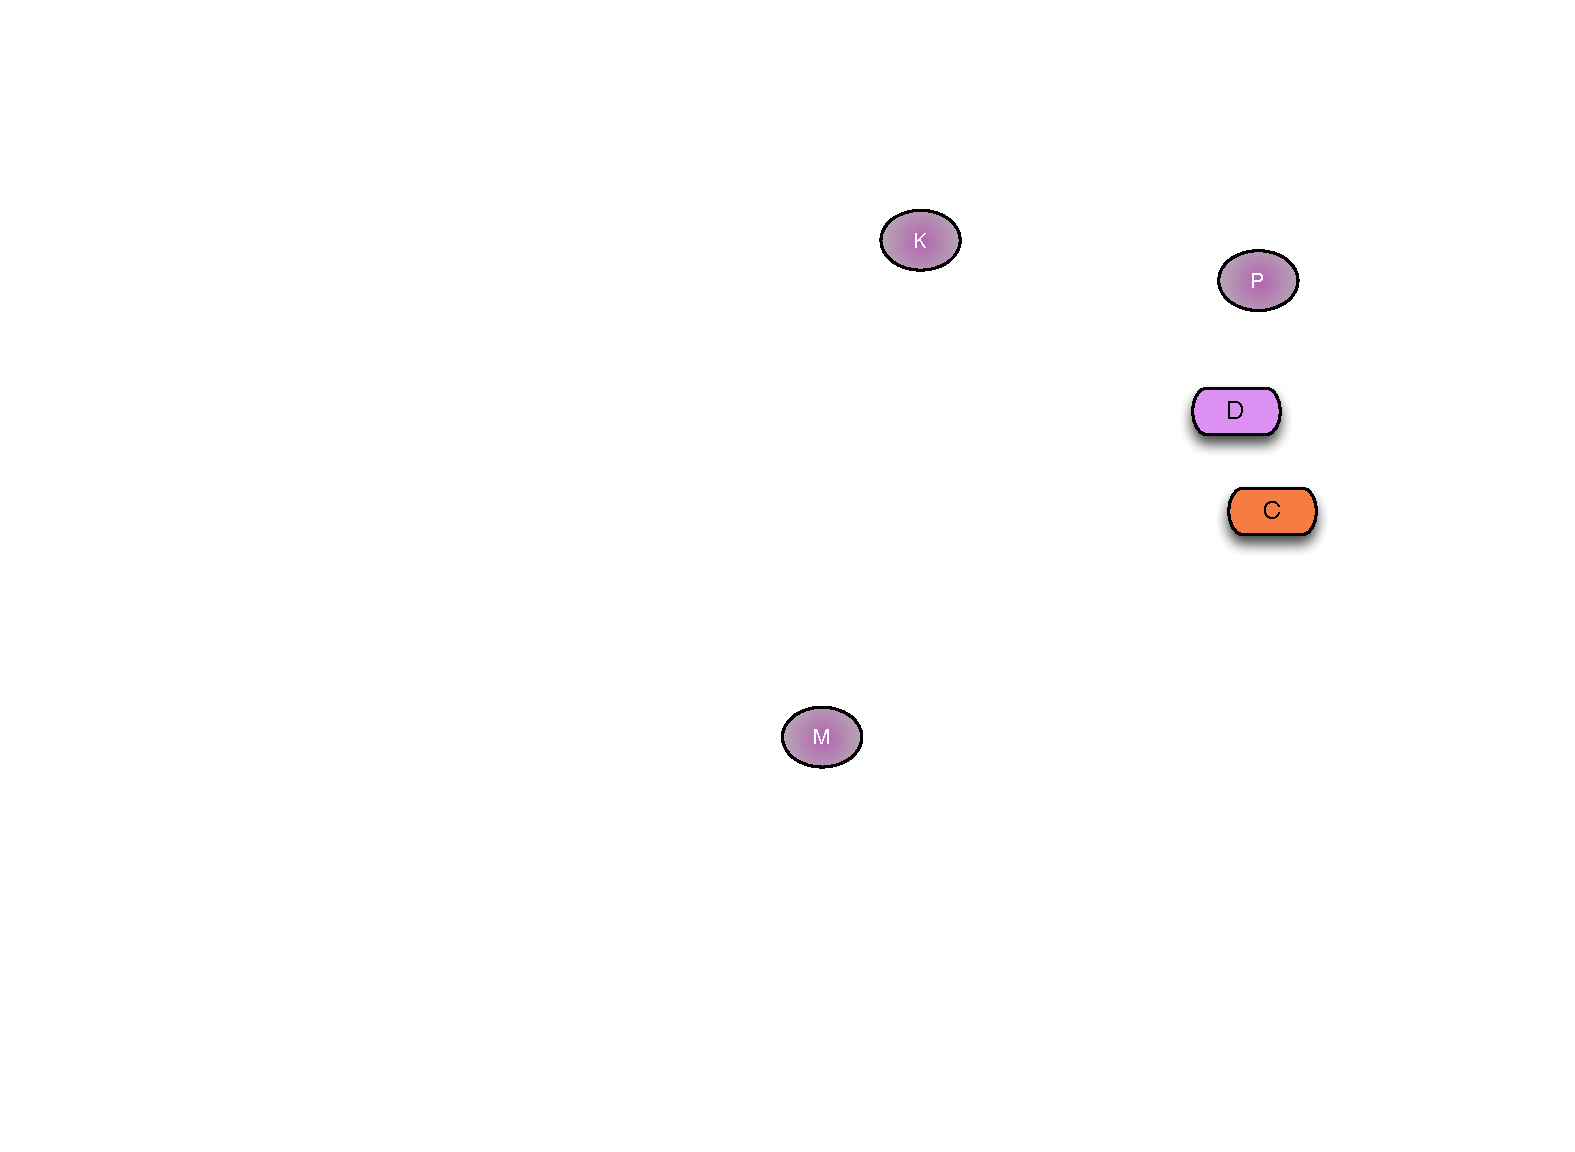
\includegraphics[width=0.9\textwidth]{../figures/progmodel/01-objects-for-algo.pdf}\end{figure}
\end{frame}


\begin{frame}
  \frametitle{Data parallelism: via an Object Collection}
  \begin{figure}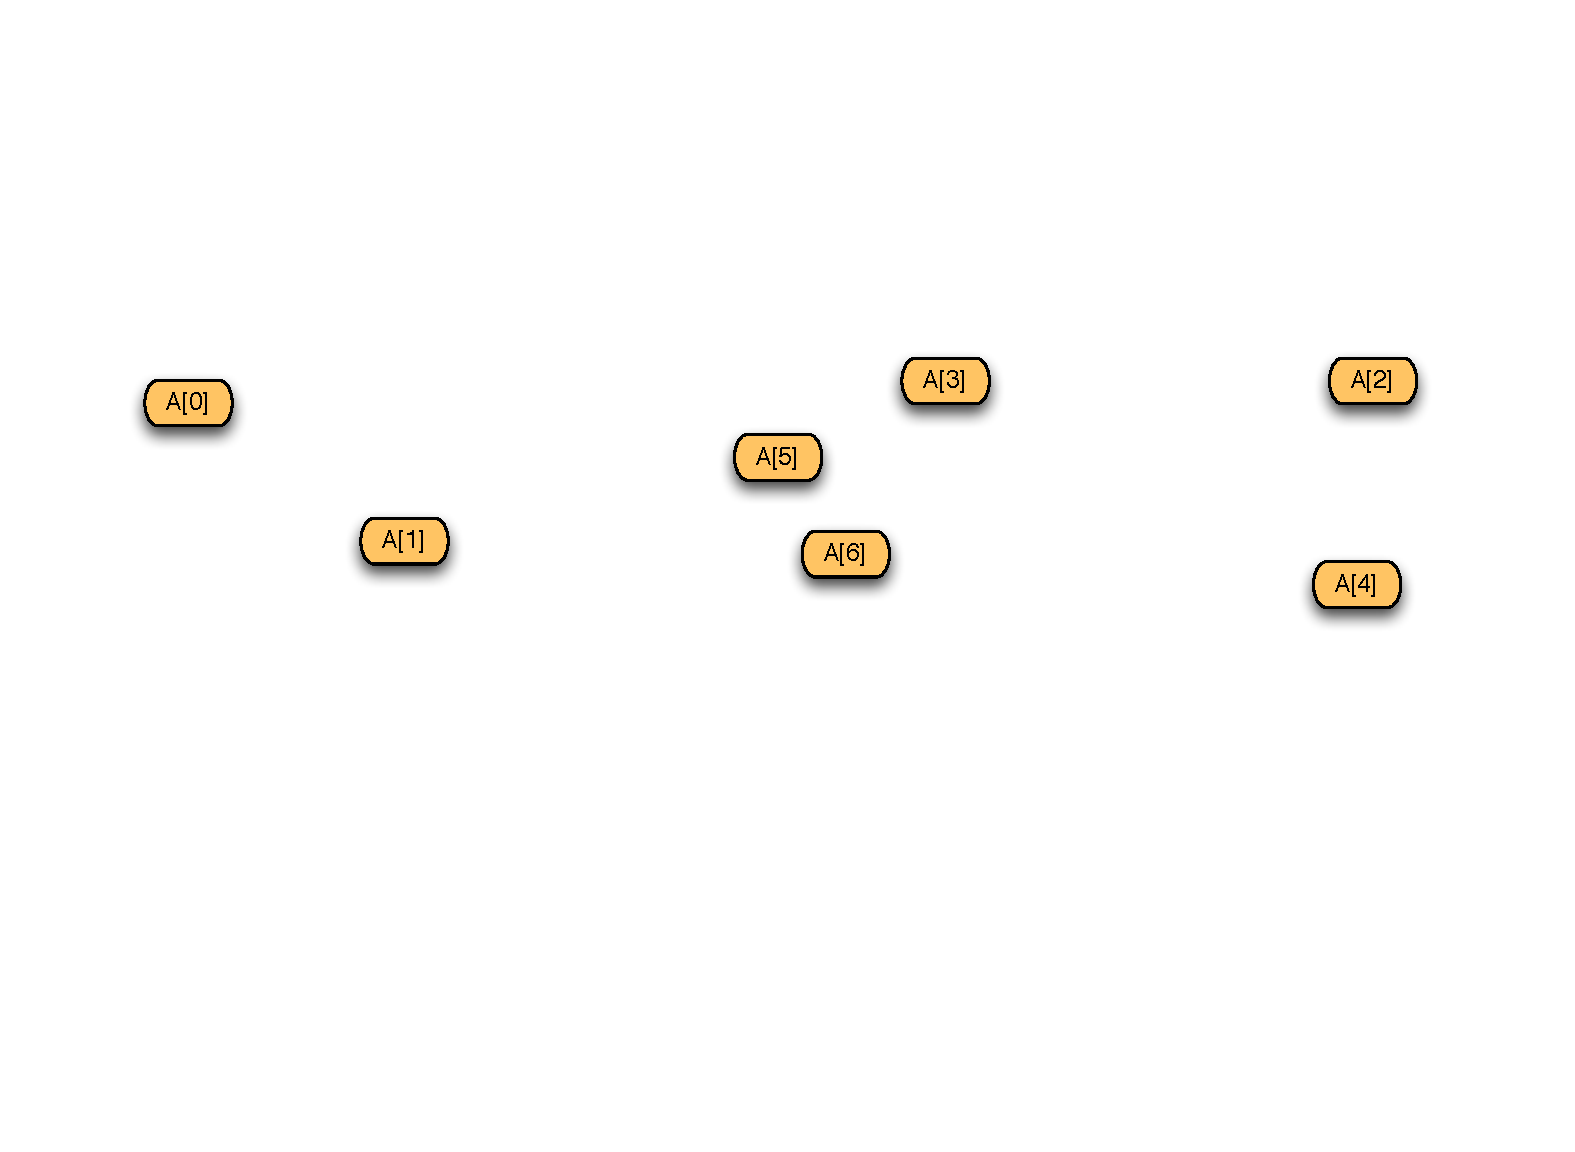
\includegraphics[width=0.9\textwidth]{../figures/progmodel/02-data-decomp-via-arrays.pdf}\end{figure}
\end{frame}


\begin{frame}
  \frametitle{Multiple data parallel collections}
say 2 matrices
  \begin{figure}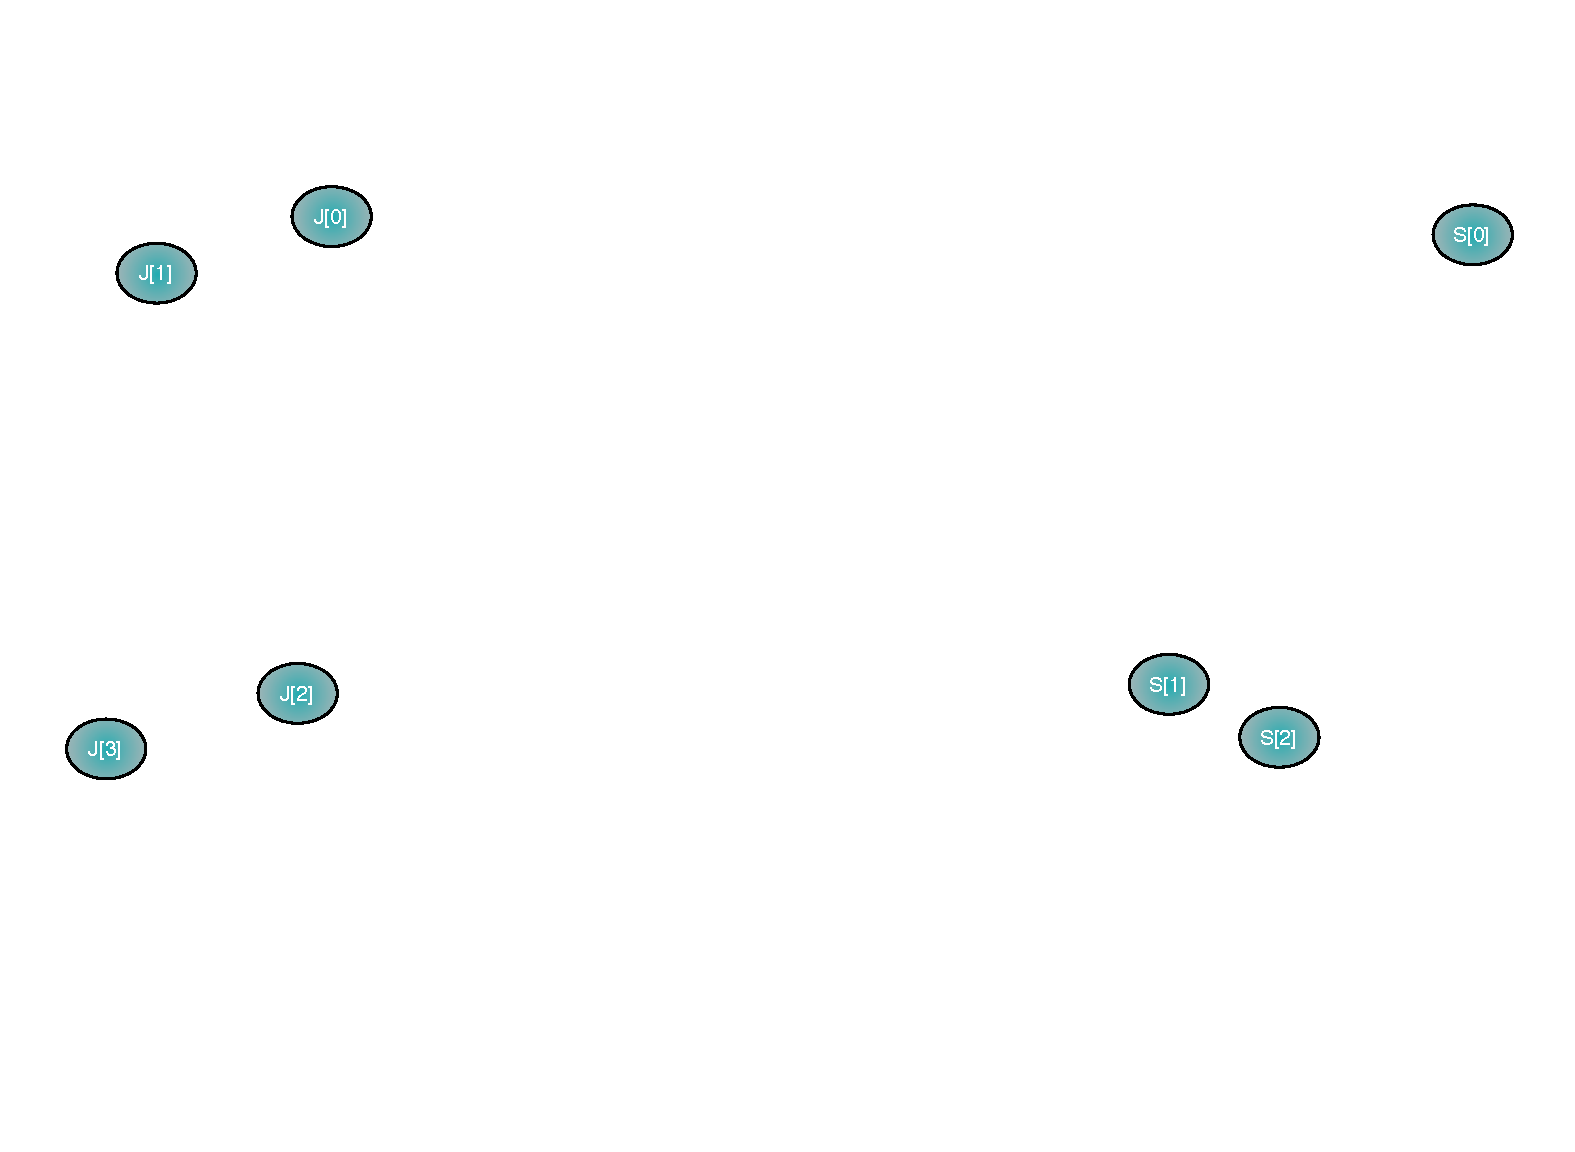
\includegraphics[width=0.9\textwidth]{../figures/progmodel/03-many-data-parallel-arrays.pdf}\end{figure}
\end{frame}


\begin{frame}
  \frametitle{Functional parallelism: via multiple classes}
  \begin{figure}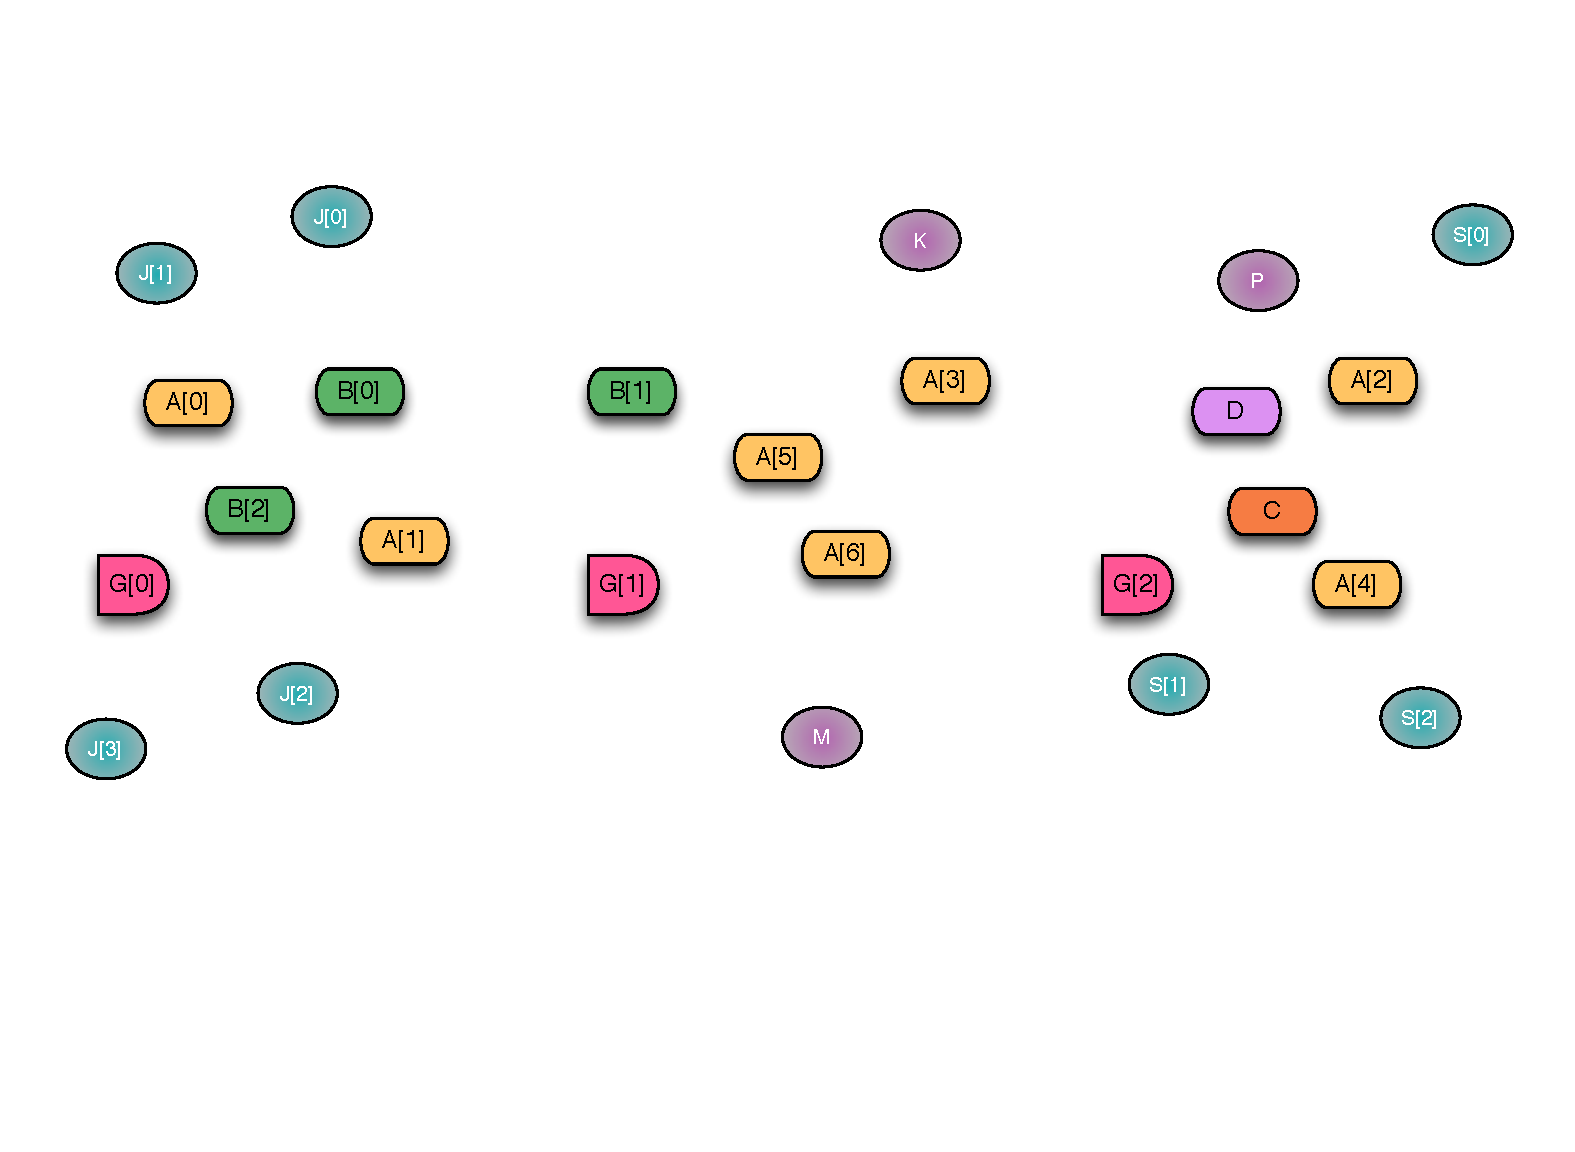
\includegraphics[width=0.9\textwidth]{../figures/progmodel/04-func-decomp-via-classes.pdf}\end{figure}
\end{frame}


\begin{frame}
  \frametitle{App logic: via classes and objects collections}
  \begin{figure}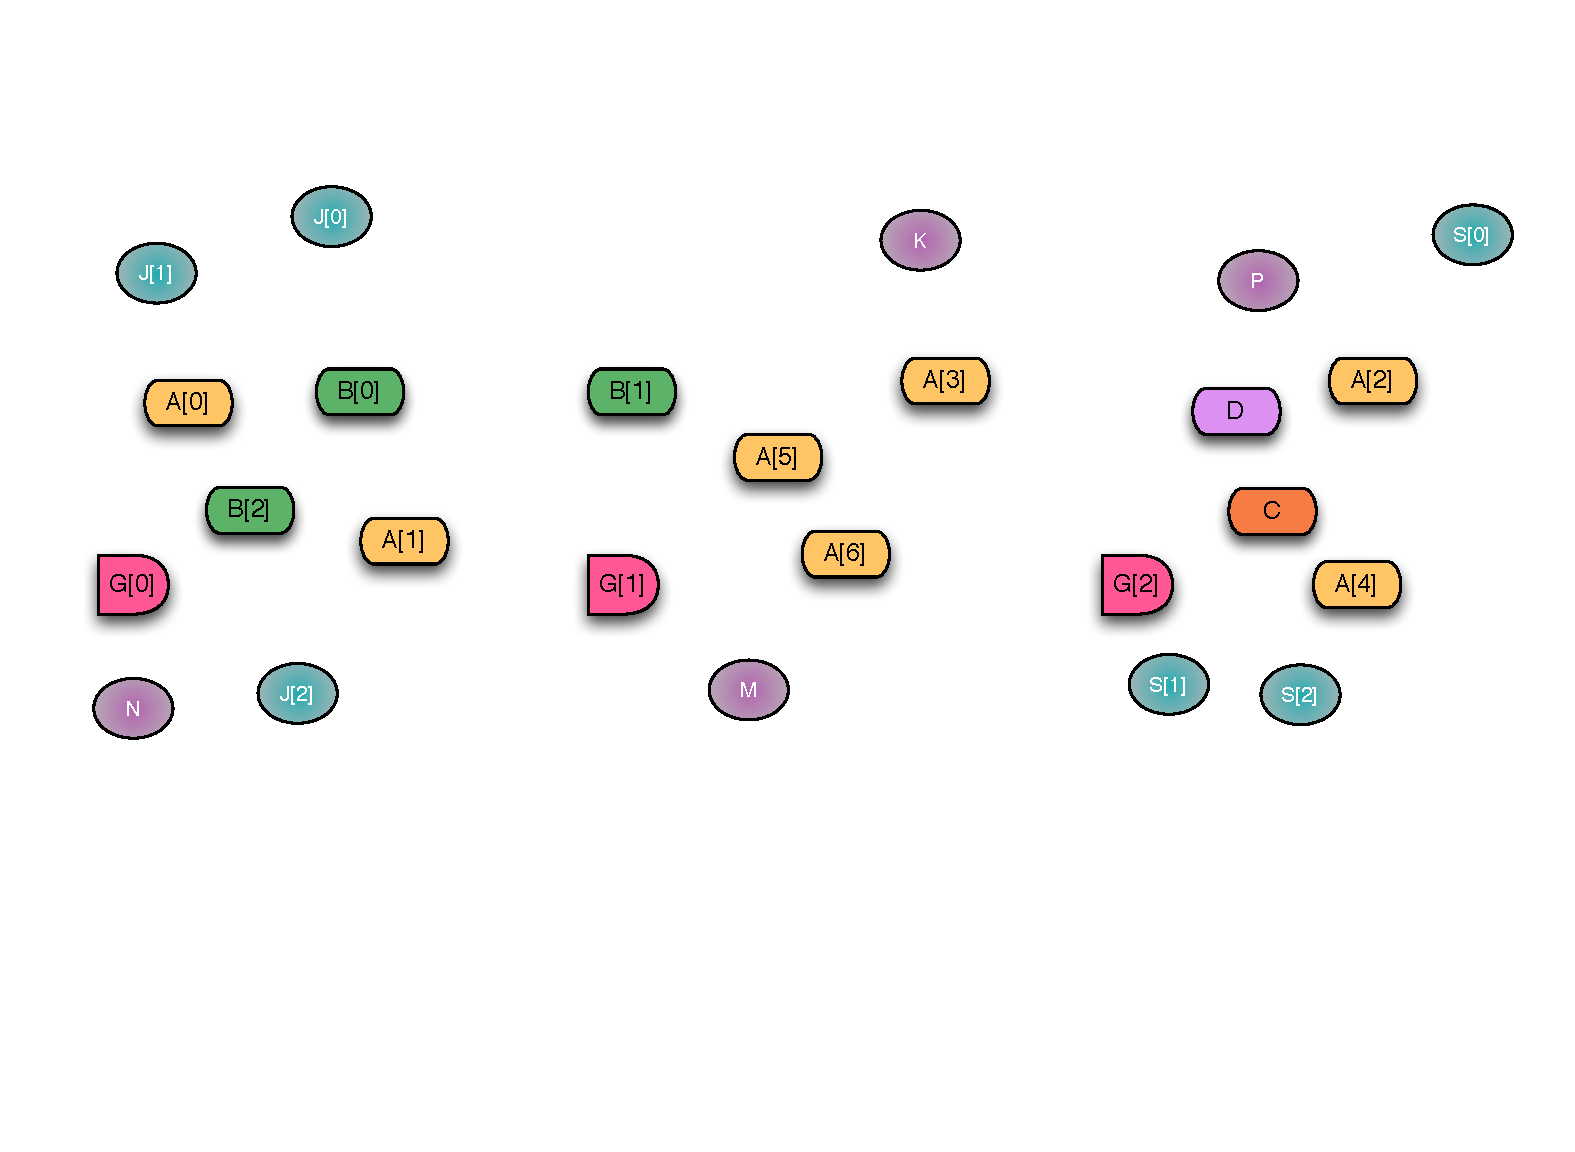
\includegraphics[width=0.9\textwidth]{../figures/progmodel/05-parallelism-via-obj-collections.pdf}\end{figure}
\end{frame}


\begin{frame}
  \frametitle{
    \only<1>{Parallelism requires distributing objects across processors}
    \only<2>{However, do not burden programmer with this view}
  }
  \begin{figure}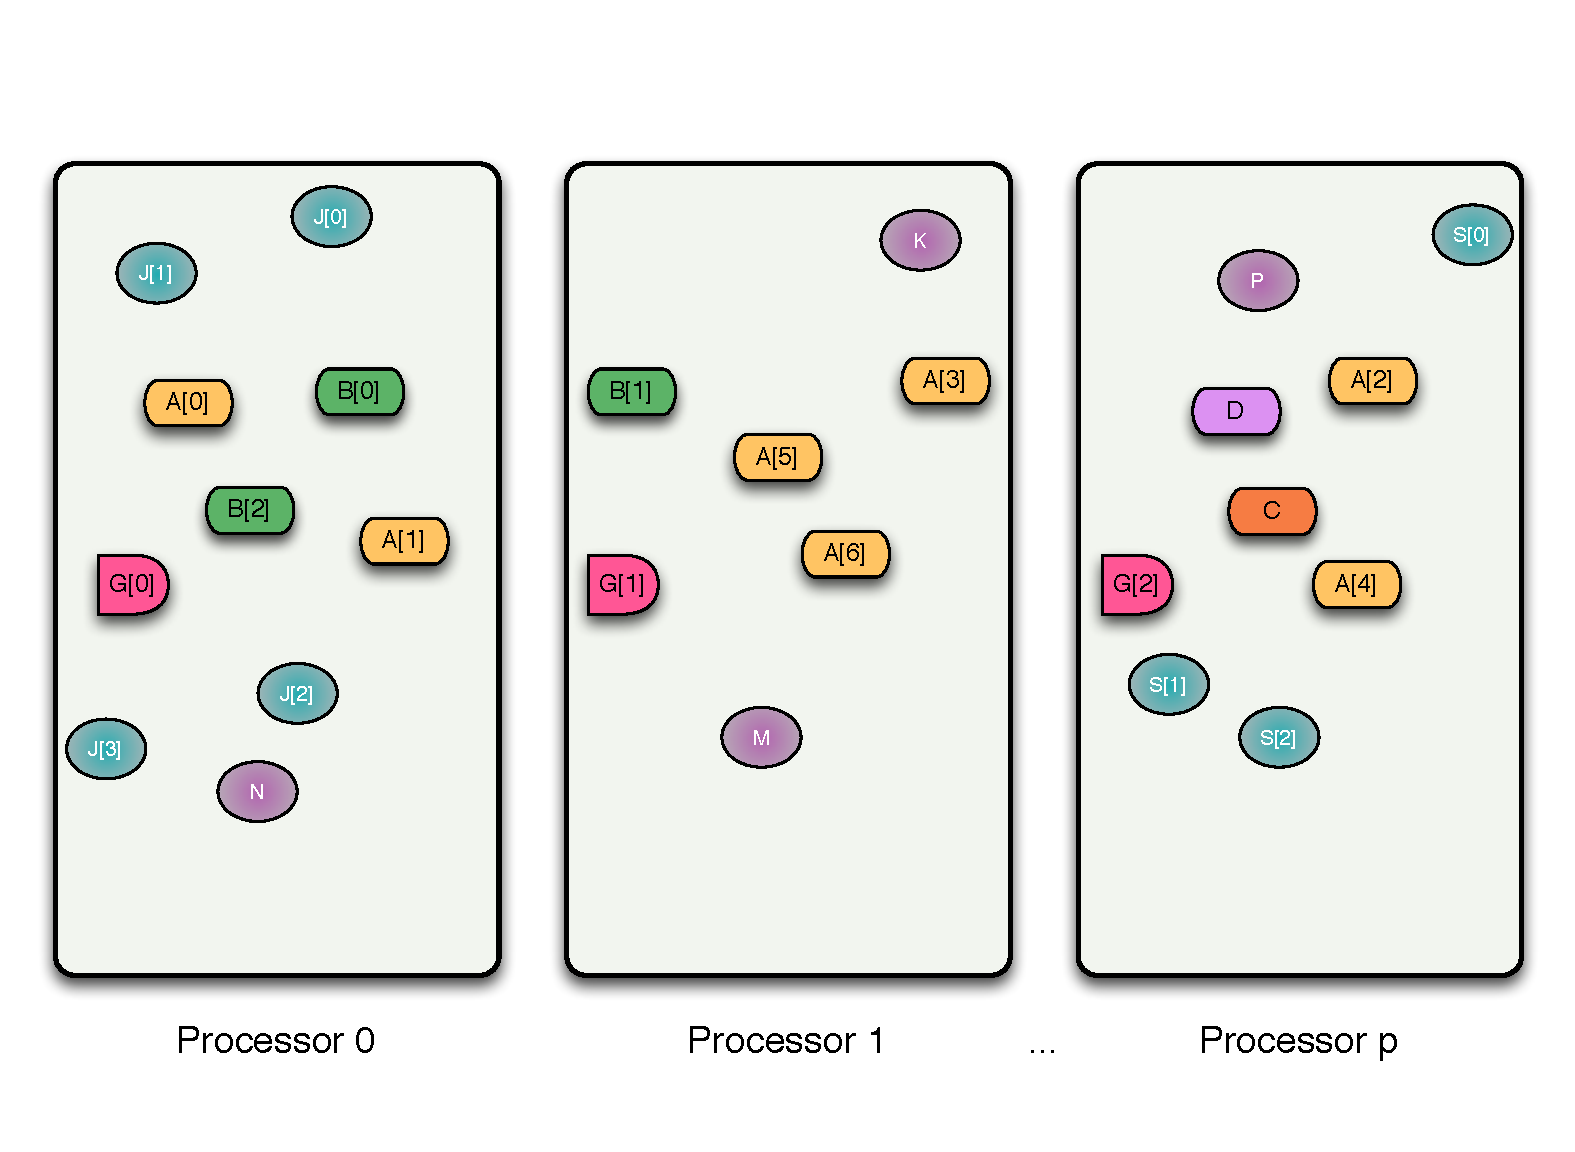
\includegraphics[width=0.9\textwidth]{../figures/progmodel/06-objects-sys-view.pdf}\end{figure}
\end{frame}


\begin{frame}
  \frametitle{
    \only<1>{Elevate some objects to global visibility}
    \only<3>{Globally visible objects = chares}
    \only<4>{Globally visible object collections = chare arrays}
  }
  \begin{figure}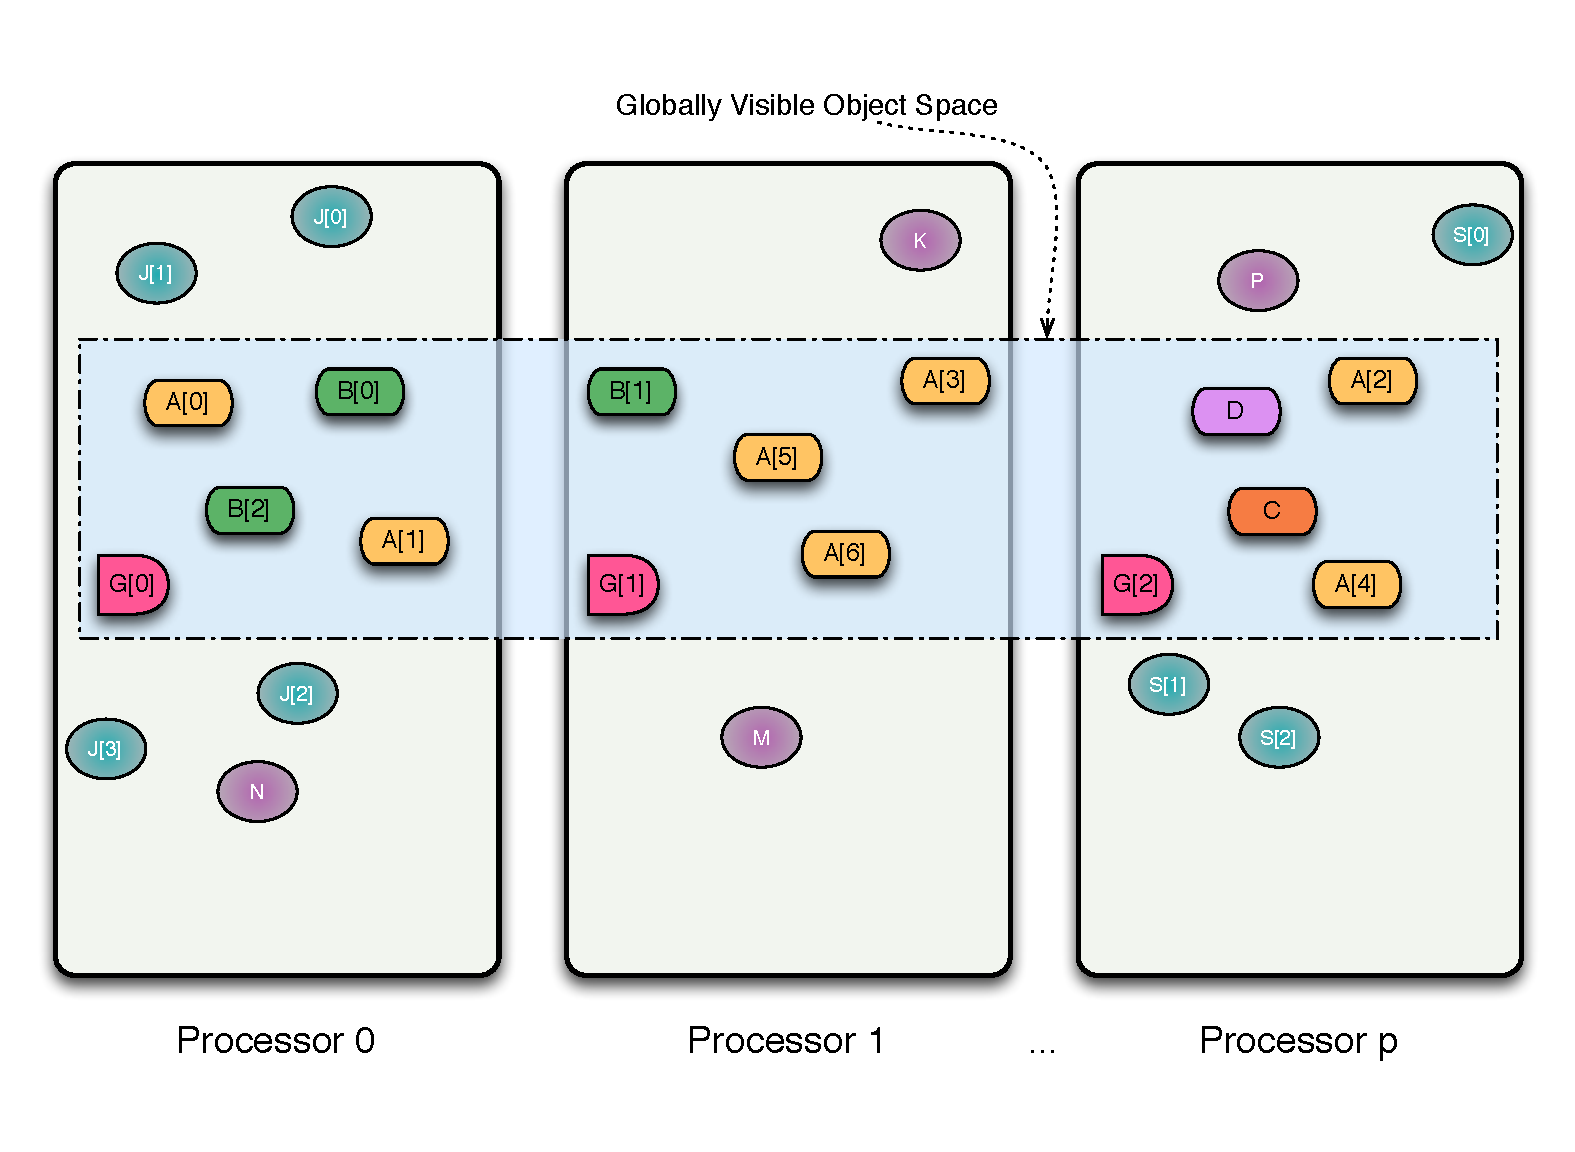
\includegraphics[width=0.9\textwidth]{../figures/progmodel/07-obj-programmer-view.pdf}\end{figure}
\end{frame}


\begin{frame}
  \frametitle{Annotating classes to enable global visibility}
  ci file declaration (just the array keyword along with dimensionality)
  class needs to inherit from generated base class
  mention code gen and promise to discuss soon
\end{frame}


\begin{frame}
  \frametitle{Addressing objects is independent of location}
  proxies. what they are. what they do. generated code.\\
  typical proxy patterns will hide the very existence of a proxy
  in that sense, this is not aptly named.
  here, it is a conscious design decision to make the user code very aware of
  the existence of the proxy. provides locality info to app programmer.
  any interaction with a proxy is a possible remote interaction.
  u can have a local instance of a chare array and access it via pointer. then local object
  but only if local. if its remote, then u have to interact via proxy
\end{frame}


\begin{frame}
\frametitle{Quantum Chemistry: OpenAtom}
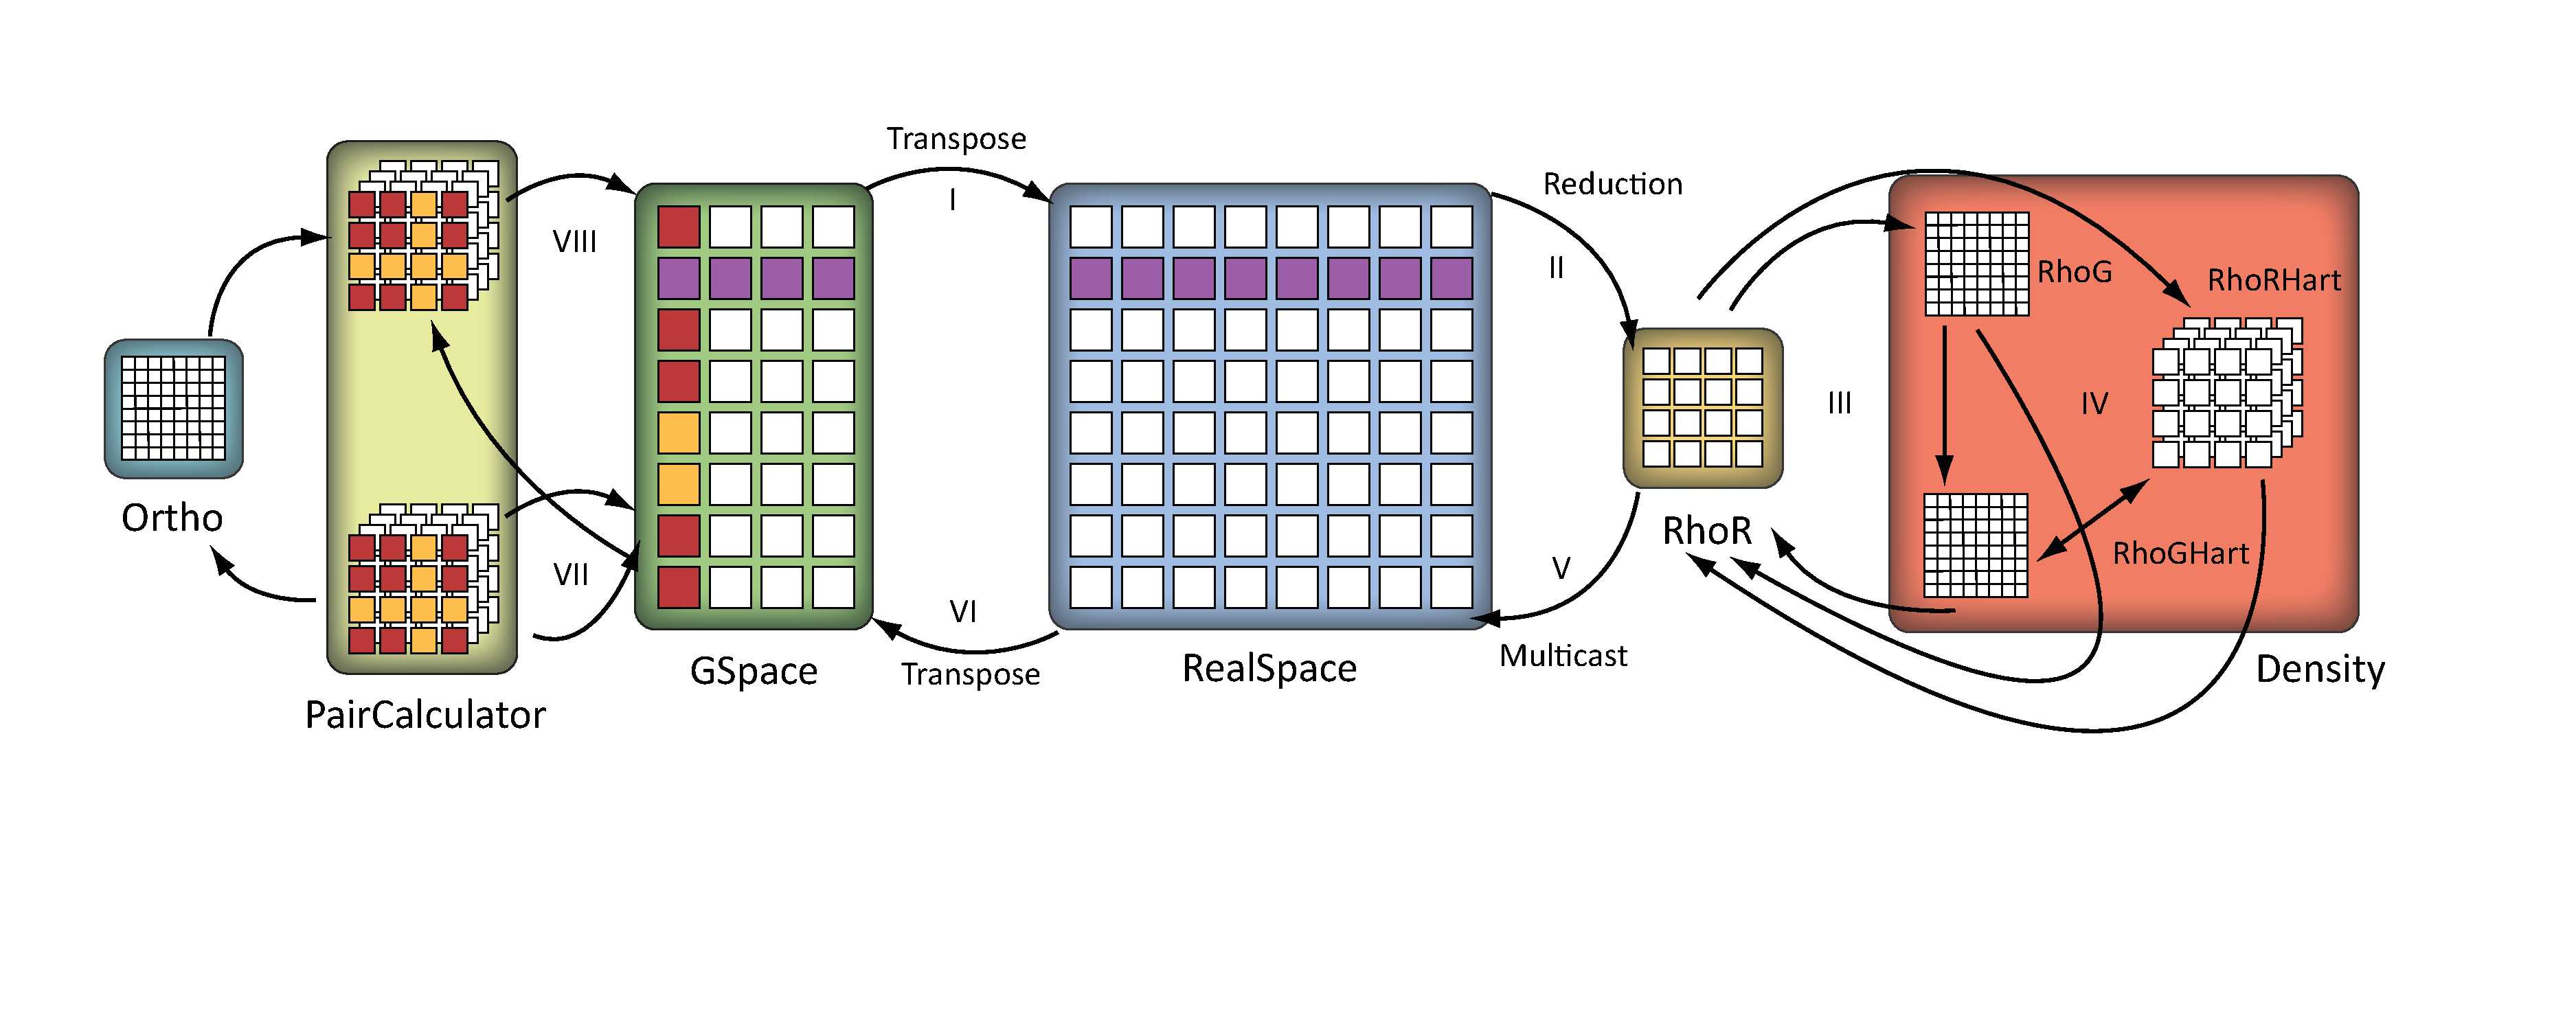
\includegraphics[width=\textwidth]{../figures/openatom/control-flow.pdf}
\end{frame}


\begin{frame}
\frametitle{Quantum Chemistry: OpenAtom}
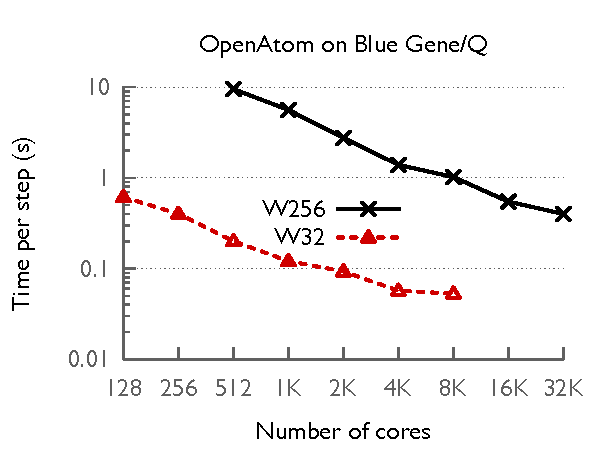
\includegraphics[width=\textwidth]{../figures/openatom/bgq.pdf}
\end{frame}


